\documentclass{beamer}
\usepackage[italian]{babel}
\usepackage[utf8]{inputenc}
\usepackage[T1]{fontenc}

% Personal commands
\newcommand{\code}[1]{\mbox{\texttt{#1}}}
\newcommand{\command}[1]{\mbox{\texttt{#1}}}
\newcommand{\file}[1]{\mbox{\texttt{#1}}}

% Beamer options
\beamertemplatenavigationsymbolsempty
\setbeamertemplate{bibliography item}{}
\setbeamertemplate{caption}{\insertcaption}
\setbeamertemplate{footline}[frame number]

\title{Web Security: introduzione al Web e HTTP}
\author[leot]{Leonardo Taccari \\ {\footnotesize \texttt{<s1069964@studenti.univpm.it>}}}
\date{}

\begin{document}

% Title of the presentation
\begin{frame}
\maketitle
\end{frame}

% Outline
\begin{frame}{Sommario}
\tableofcontents
\end{frame}

\section{World Wide Web}
\begin{frame}{\insertsection}
\end{frame}

\begin{frame}{\insertsection}
\begin{itemize}
\item \alert{World Wide Web}, AKA \alert{WWW}, AKA \alert{Web}~\footnote{Lo chiameremo
semplicemente Web a seguire.}
\item È una \alert{collezione globale di documenti} e altre risorse, collegate da
\alert{hyperlinks} e \alert{URL}.
\item I documenti vengono scambiati attraverso il protocollo di comunicazione
\alert{HTTP}
\item La maggior parte dei documenti sono degli \alert{ipertesti} scritti nel
linguaggio \alert{HTML}
\end{itemize}
\end{frame}

\subsection*{Un po' di storia}
\begin{frame}{\insertsection}{\insertsubsection}
\begin{itemize}
\item Proposto da Tim Berners-Lee al CERN nel 1989 e rilasciato pubblicamente nel 1993
\item Nel 1994 viene fondato il World Wide Web Consortium (W3C) che si occupa
degli standard che costituiscono il Web
\item Inizialmente nato per scambiare \alert{ipertesti}, poi \alert{ipermedia}
\item \alert{Web 1.0}, \alert{web statico}, l'utente può esclusivamente leggere i
contenuti senza possibilità di modificarli
\item \alert{Web 2.0}, \alert{web dinamico}, l'utente può anche modificare i
contenuti
\end{itemize}
\end{frame}

\subsection*{Home page del primo sito web della storia}
\begin{frame}{\insertsection}{\insertsubsection}
\begin{figure}
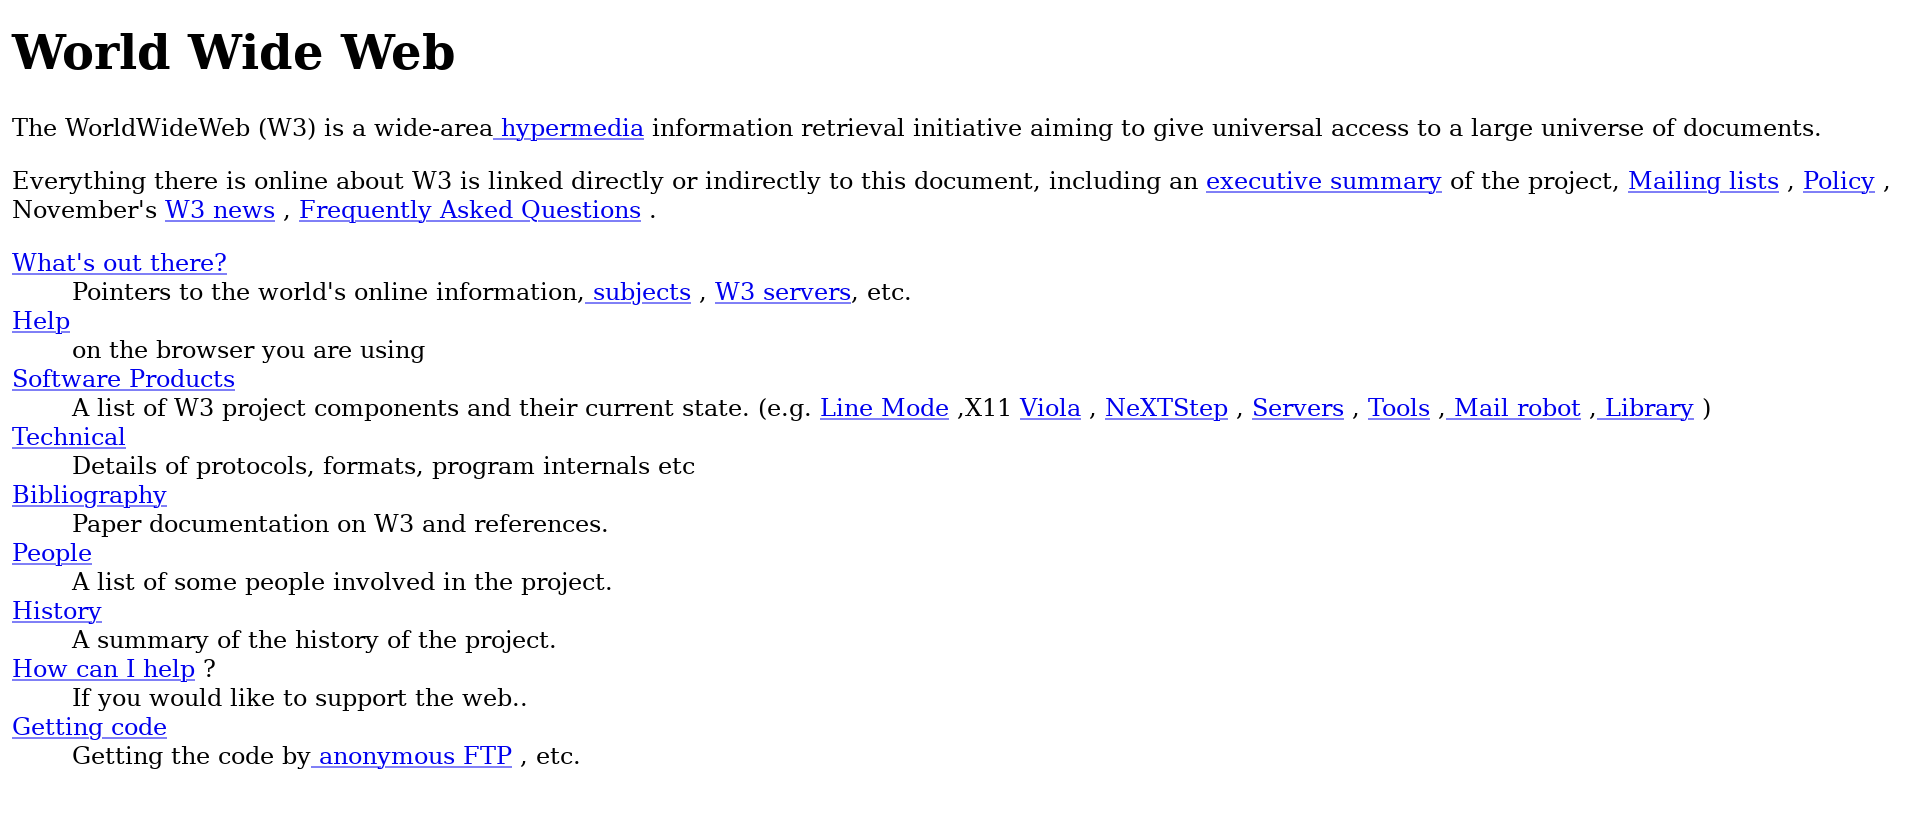
\includegraphics[width=0.95\textwidth]{imgs/www-historical-page-screenshot.png}
\caption{Home page del primo sito web della storia, pubblicato il 20 dicembre
1990 su \url{https://info.cern.ch/hypertext/WWW/TheProject.html}
\href{https://web.archive.org/web/20250129055359/https://info.cern.ch/hypertext/WWW/TheProject.html}{(capture da Wayback Machine dell'Internet Archive)}}
\end{figure}
\end{frame}

\section{Uniform Resource Locator (URL)}
\begin{frame}{\insertsection}
\begin{itemize}
\item Ogni risorsa nel Web è identificata da un indirizzo detto
\alert{Uniform Resource Locator (URL)}
\item Ad esempio, \url{https://www.example.org/index.html} identifica
l'\alert{home page} di \alert{www.example.org}
\item Nel \alert{browser web} l'URL viene mostrato in una barra
\end{itemize}
\end{frame}

\subsection*{Anatomia di un URL}
\begin{frame}[allowframebreaks]{\insertsection}{\insertsubsection}
\begin{itemize}
\item Un \alert{URL} è costituito da diverse parti
\item La sintassi generale è
\small{\code{scheme://[userinfo@]host[:port][path][?query][\#fragment]}}
\begin{description}
\item[scheme] indica il protocollo utilizzato, ad esempio \code{http} o
\code{https}
\item[userinfo] (opzionale) solitamente nel formato
\code{username:password} utilizzata per accedere a risorse che richiedono delle
credenziali
\item[host] hostname o indirizzo IP
\item[port] (opzionale) port, di default 80 per HTTP e 443 per
HTTPS~\footnote{Vedremo meglio ciò in Network Security!}
\item[path] (opzionale) "percorso", ogni componente è prefissato da un \code{/}
\item[query] (opzionale) "query string", costituisce coppie attributi-valori
separati da \code{\&}, solitamente utilizzate per sottomettere dati
\item[fragment] (opzionale) identifica un determinato frammento all'interno
della risorsa (ad esempio permette di "evidenziare" una parte di testo)
\end{description}
\item Esempio: \url{https://www.example.org/index.html}
\begin{description}
\item[https] è lo \alert{schema} seguito da \code{:}
\item[www.example.org] è l'\alert{host} prefissato da \code{//}
\item[/index.html] è il \alert{path} costituito da un singolo componente
\end{description}
\end{itemize}
\end{frame}

\section{HyperText Transfer Protocol (HTTP)}
\begin{frame}{\insertsection}
\begin{itemize}
\item \alert{HyperText Transfer Protocol (HTTP)} è il protocollo di
comunicazione utilizzato per scambiarsi risorse nel Web
\item Basato sul modello \alert{client-server}: la comunicazione viene iniziata
dal \alert{client} che \alert{richiede} una \alert{risorsa} al \alert{server} che a sua
volta fornisce al client la risorsa in una \alert{risposta}
\item L'applicazione client HTTP viene detta \alert{browser web}
\item L'applicazione server HTTP viene detta \alert{web server}
\end{itemize}
\end{frame}

\subsection*{Flusso di una richiesta e risposta HTTP}
\begin{frame}{\insertsection}{\insertsubsection}
\begin{itemize}
\item Vediamo il flusso di richiesta e risposta HTTP
\item Come esempio pratico ci chiediamo che cosa succede quando
scriviamo nella barra del browser
\url{https://www.kittenwar.com/c\_images/2006/08/10/84180.1.jpg}
\end{itemize}
\end{frame}

\subsubsection*{Digitazione dell'URL nel browser}
\begin{frame}{\insertsubsection}{\insertsubsubsection}
\begin{figure}
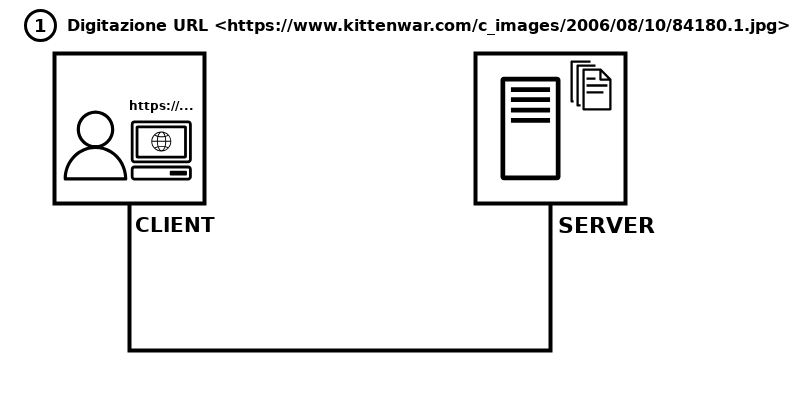
\includegraphics[width=0.88\textwidth]{imgs/http-kittenwar-1.png}
\caption{Digitiamo nel browser web l'URL all'immagine di Joe Dirt}
\end{figure}
\end{frame}

\subsubsection*{Richiesta HTTP}
\begin{frame}{\insertsubsection}{\insertsubsubsection}
\begin{figure}
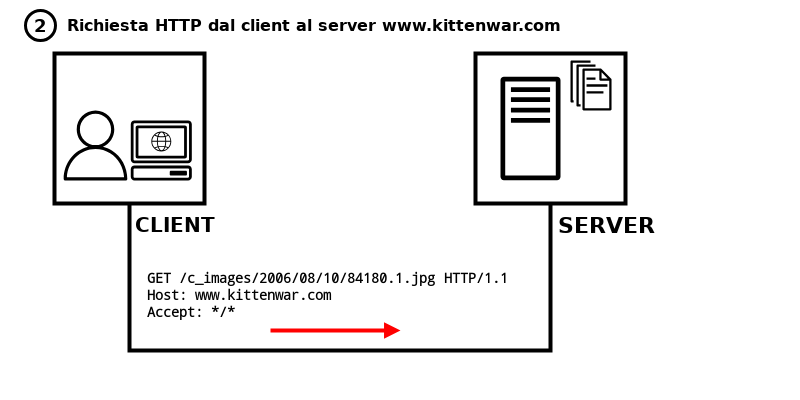
\includegraphics[width=0.88\textwidth]{imgs/http-kittenwar-2.png}
\caption{Il browser spedisce al server la richiesta HTTP per ottenere la
risorsa}
\end{figure}
\end{frame}

\subsubsection*{Risposta HTTP}
\begin{frame}{\insertsubsection}{\insertsubsubsection}
\begin{figure}
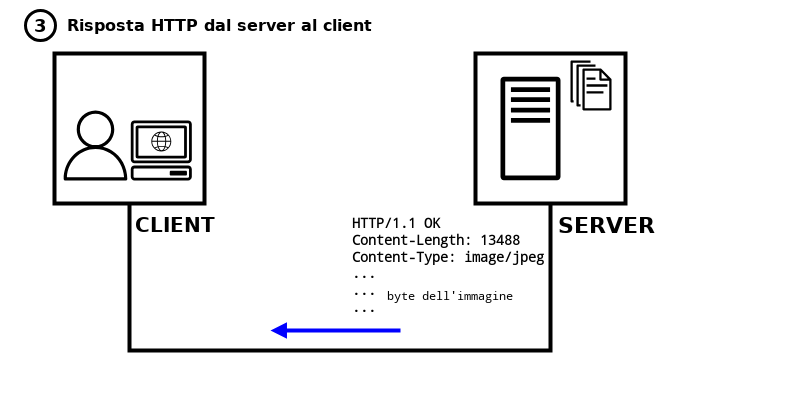
\includegraphics[width=0.88\textwidth]{imgs/http-kittenwar-3.png}
\caption{Il server web restituisce in risposta la risorsa richiesta}
\end{figure}
\end{frame}

\subsubsection*{Rendering dell'immagine nel browser}
\begin{frame}{\insertsubsection}{\insertsubsubsection}
\begin{figure}
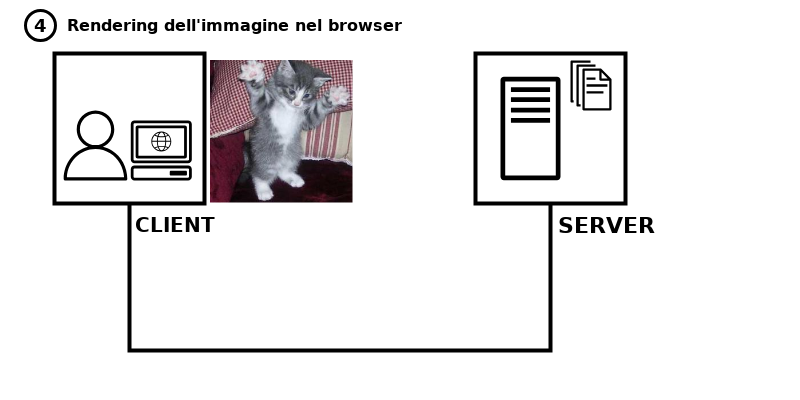
\includegraphics[width=0.88\textwidth]{imgs/http-kittenwar-4.png}
\caption{L'immagine viene visualizzata nel browser web}
\end{figure}
\end{frame}

\subsection*{Messaggio HTTP}
\begin{frame}{\insertsection}{\insertsubsection}
\begin{itemize}
\item Le richieste e le risposte HTTP sono dei \alert{messaggi HTTP}
\item I messaggi HTTP hanno la seguente struttura:
\begin{description}
\item[riga iniziale (start line)] indica la versione HTTP e il metodo della
richiesta (per richieste) o lo status della risposta (per risposte)
\item[header] metadata che descrivono il messaggio
\item[riga vuota (empty line)] riga vuota (CRLF, carrige return e line feed)
che separa l'header dal body
\item[body] (opzionale) contenuto del messaggio
\end{description}
\end{itemize}
\end{frame}

\subsection*{Richiesta HTTP}
\begin{frame}[allowframebreaks]{\insertsection}{\insertsubsection}
\begin{itemize}
\item Spedita dal \alert{client} al \alert{server}
\item È costituita da:
\begin{description}
\item[request-line] contiene la tripletta \alert{metodo (method)},
\alert{request-target} e \alert{protocollo (protocol)}
\begin{description}
\item[metodo (method)] metodo (detto anche verbo), ad esempio:
\code{GET} (per ricevere una risorsa) o \code{POST} (per spedire dati)
\item[request-target] solitamente un URL relativo (senza dominio)
\item[protocollo (protocol)] versione del protocollo HTTP utilizzata
\end{description}
\item[request header] metadati, \code{Host:} è l'unico sempre richiesto, si
suddividono in \alert{request header} e \alert{representation header}
\item[body] (opzionale) contenuto della richiesta
\end{description}
\end{itemize}
\end{frame}

\subsection*{Risposta HTTP}
\begin{frame}[allowframebreaks]{\insertsection}{\insertsubsection}
\begin{itemize}
\item Spedita dal \alert{server} al \alert{client}
\item È costituita da:
\begin{description}
\item[status line] contiene la tripletta \alert{protocollo (protocol)},
\alert{status code} e \alert{status text}
\begin{description}
\item[protocollo (protocol)] versione del protocollo HTTP utilizzata
\item[status code] codice numerico che indica l'esito della richiesta, ad
esempio $200$, $403$, $404$, $503$~\footnote{Diversi status code sono
rappresentati in \url{https://http.cat}}
\item[status text] descrizione testuale dello status code
\end{description}
\item[response header] metadati della risposta, si suddividono \alert{response
header} e \alert{representation header}
\item[body] (opzionale) contenuto della risposta
\end{description}
\end{itemize}
\end{frame}

\subsection*{Un po' di pratica!}
\begin{frame}{\insertsection}{\insertsubsection}
\begin{itemize}
\item \alert{curl} è un client \alert{HTTP}
\item Non è un vero e proprio browser: non permette di visualizzare gli
ipermedia ma ci permette di effettuare richieste HTTP e visualizzare la
risposta HTTP
\item È molto potente ed utile sia per capire HTTP che per risolvere challenge
\item Leggiamo velocemente la pagina di manuale \code{curl(1)} con
\command{man curl}
\item Vediamo e commentiamo insieme
\small{\command{curl --http1.1 --verbose http://www.example.org/index.html}}
\end{itemize}
\end{frame}

\section{Conclusioni}
\begin{frame}{\insertsection}
\begin{itemize}
\item Abbiamo visto che cosa è il \alert{World Wide Web} e la sua storia
\item Abbiamo visto che cosa sono gli \alert{URL}, gli identificatori di risorse
alla base del Web
\item Abbiamo visto il protocollo di comunicazione \alert{HTTP} e visto in
dettaglio - ed anche in pratica! - le richieste e risposte HTTP
\end{itemize}
\end{frame}

% FIXME: Use bibtex for that!
\section{Riferimenti}
\begin{frame}{\insertsection}
\begin{itemize}
\item \href{https://training.olicyber.it/training}{Materiale Didattico del Portale di allenamento delle Olimpiadi Italiane di Cybersicurezza} 
\item \href{https://developer.mozilla.org/en-US/}{MDN Web Docs} 
\end{itemize}
\end{frame}

\end{document}
